\part{Введение в математический анализ}
\chapter[Теорема Больцано-Вейерштрасса и критерий Коши сходимости числовой последовательности.]{Теорема Больцано-Вейерштрасса и критерий Коши сходимости числовой последовательности.}

\section[Аксиоматика множества действительных чисел]{Аксиоматика множества действительных чисел\footnote{\leavevmode\vspace*{-\baselineskip}
\InsertBoxL{0}{\llap{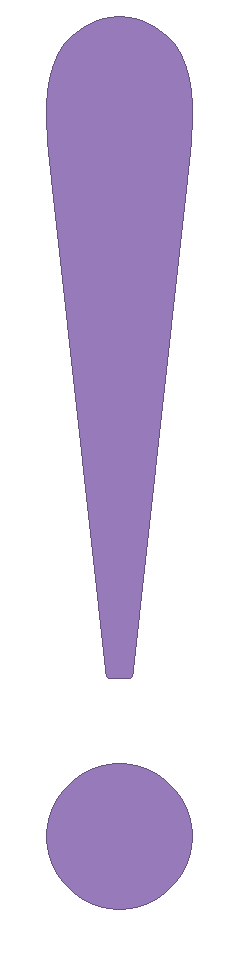
\includegraphics[height=2.5cm]{Bang}}}%
\mbox{\kern0.1em}
Необходимо сразу предостеречь читателя, что данное пособие является именно кратким пересказом курса математики на физтехе, охватывающим вопросы к ГОСу. Пересказ должен быть цельным, а не отрывочным "--- как предлагает программа ГОСа, поэтому материал в билетах порой является избыточным для рассказа билета на самом экзамене. Например, я бы не стал первый говорить о аксиоматике множества действительных чисел, однако поместить ее в это место в книге я просто обязан для полной картины мира, поскольку это, как уже было сказано выше, лишь конспект высшей математики на Физтехе. Однако оставляю читателю полную свободу выбора тем разговора с преподавателем. Я хочу сказать, что названия глав это лишь названия билетов, контрольные точки, к которым плавно материал книги пытается подвести читателя.
}
}

\begin{defn}
Будем говорить, что на множестве $X$ определена операция сложения <<$+$>> (умножения <<$\cdot$>>), если любой упорядоченной паре элементов $(a,b)$ элементов $X$ поставлен в соответствие элемент $y = a + b$ ($y = a\cdot b$)
\end{defn}

Зачастую знак умножения <<$\cdot$>> опускают и пишут $ab$ вместо $a\cdot b$.

\begin{defn}
Будем говорить, что на множестве $X$ задано отношение порядка <<$\le$>>, если для любых двух элементов $a,b\in X$ выполняется хотя бы одно из условий $a\le b$, $b \le b$.
\end{defn}

Другими словами, для любых $a, b \in \bbR$ заранее установлено, верно или неверно неравенство $a \le b$ (или $b \le a$).

\begin{defn}
Множество $\bbR$, состоящее более, чем из одного элемента, называется \textit{множеством действительных (вещественных) чисел}, а его элементы "--- \textit{действительными (вещественными) числами}, если на $\bbR$ определены операции сложения~<<$+$>> и умножения~<<$\cdot$>> и отношение порядка~<<$\le$>>, удовлетворяющие следующим 15 аксиомам\rindex{аксиомы!множества действительных чисел}:
\end{defn}

\begin{enumerate}[label=\Roman*.]
\item
\textbf{Аксиомы сложения} (\,$+\colon a,b \to a+b$\,)
\begin{enumerate}[label=\arabic*.]
\item 
$a + b = b + a\quad\forall a,b \in \bbR$ (коммутативность);
\item
$a + (b + c) = (a + b) + c\quad \forall a,b,c \in \bbR$ (ассоциативность);
\item
$\exists 0 \in \bbR\cquad a + 0 = a\quad \forall a \in \bbR$;
\item 
$\forall a \in \bbR \quad \exists (-a) \in \bbR\cquad a + (-a) = 0$, $(-a)$ называется \textit{противоположным} числом для $a$.
\end{enumerate}
\item
\textbf{Аксиомы умножения} (\,$\cdot\colon a,b \to a\cdot b$)
\begin{enumerate}[resume, label=\arabic*.]
\item
$a\cdot b = b \cdot a \quad \forall a,b\in \bbR$ (коммутативность);
\item
$a \cdot (b \cdot c) = (a \cdot b) \cdot c\quad \forall a,b,c \in \bbR$ (ассоциативность);
\item 
$\exists 1 \in \bbR,\ 1\ne 0\cquad a\cdot1 = a\quad \forall a\in \bbR$;
\item 
$\forall a\in \bbR,\ a\ne 0,\quad \exists \frac{1}{a} \in \bbR\cquad a\cdot \frac{1}{a} = 1$, $\frac{1}{a}$ называется \textit{противоположным} числом для $a$.
\end{enumerate}
\item
\textbf{Аксиома связи сложения и умножения}
\begin{enumerate}[resume, label=\arabic*.]
\item
$(a+b) \cdot c = a\cdot c +  b\cdot c\quad \forall a,b,c \in \bbR$ (дистрибутивность умножения относительно сложения).
\end{enumerate}
\item
\textbf{Аксиомы порядка} 
\begin{enumerate}[resume, label=\arabic*.]
\item 
$ a \le a\quad \forall a \in \bbR$;
\item
$ a\le b,\ b\le a \Rightarrow a=b \quad \forall a,b\in\bbR$;
\item
$a\le b,\ b\le c \Rightarrow a\le c\quad \forall a,b,c\in \bbR$ (транзитивность).
\end{enumerate}
\item
\textbf{Аксиома связи сложения и порядка}
\begin{enumerate}[resume, label=\arabic*.]
\item 
$ a \le a\Rightarrow a + c \le b + c\quad \forall a,b,c \in \bbR$.
\end{enumerate}
\item
\textbf{Аксиома связи умножения и порядка}
\begin{enumerate}[resume, label=\arabic*.]
\item 
$ 0 \le a,\ 0\le b\Rightarrow 0 \le a\cdot b\quad \forall a,b \in \bbR$.
\end{enumerate}
\item
\textbf{Принцип непрерывности}
\begin{enumerate}[resume, label=\arabic*.]
\item 
Пусть $A$, $B$ "--- непустые подмножества $\bbR$ такие, что
$$
a\le b\quad \forall a \in A, \  \forall b \in B.
$$
Тогда $\exists c \in \bbR$ такое, что $a\le c\le b\quad \forall a \in A,\ \forall b\in B.$
\end{enumerate}
\end{enumerate}
\enlargethispage{\baselineskip}
\begin{defn}
Определим отношения порядка <<$<$>>, <<$>$>>, <<$\ge$>> и операции вычитания~<<$-$>> и деления~<<$/$>> на множестве $\bbR$:
\begin{itemize}[noitemsep,  topsep=0pt]
\item 
$a < b \Longleftrightarrow a \le b \text{ и } a\neq b$;
\item
$a > b \Longleftrightarrow b < a$, аналогично $a \ge b \Longleftrightarrow b \le a$;
\item
$a - b \triangleq a + (-b)$;
\item
$a / b =  \frac{a}{b} \triangleq a \cdot \frac{1}{b}$; 
\end{itemize}
\end{defn}


\begin{defn}
Напоследок, определим некоторые важнейшие числовые множества:
\begin{itemize}[wide, labelwidth=!, labelindent=0pt, nolistsep, topsep=0pt]
\item 
Множество \textit{натуральных} чисел $$\bbN = \{1,\ 1+1=2,\ \dots\,,\ n = 1+\dots+1,\ \dots\,\}.$$
\item 
Множество $\bbN_0 \triangleq \bbN \cup \{0\}.$
\item 
Множество \textit{целых} чисел $$\bbZ = \{ 0,\ 1,\ -1,\ 2,\ -2,\ 3,\ -3,\ \dots\,\},$$ т.е.\ множество чисел $x$ таких, что $x\in \bbN$ или $-x \in \bbN$, или $x = 0$.
\item
Множество \textit{рациональных} чисел $$\bbQ=\{\,x\,\big|\,x=p/q,\ q\in\bbN,\ p\in\bbZ\,\}.$$
\item 
Множество \textit{иррациональных чисел} $\bbR \setminus \bbQ$.
\item 
Множество действительных чисел $\bbR$ часто называют \textit{числовой прямой}, а числа "--- \textit{точками числовой прямой}. А сами действительные числа часто будем называть \textit{числами}, подразумевая именно элементы из множества~$\bbR$.
\item 
Наряду с числовой прямой определим \textit{расширенную числовую прямую:} множество $\bboR=\bbR\cup \{-\infty, {+\infty}\}$. В нем определены отношения порядка, операции <<$+$>>, <<$\cdot$>> для элементов из $\bbR$. Элементы $-\infty$, $+\infty$ не содержатся в $\bbR$. Для них определены отношения порядка: $\forall x \in \bbR$\quad$-\infty < x < +\infty$. Частично определены операции <<$+$>>, <<$-$>>, <<$\cdot$>> и <<$/$>>:
\begin{align*}
&+\infty + a = +\infty \quad\text{и}\quad +\infty - a = +\infty,\quad \forall a \in \bbR\cup\{+\infty\}; \\
&-\infty - a = -\infty \quad\text{и}\quad -\infty + a = -\infty,\quad \forall a \in \bbR\cup\{-\infty\}; \\
&+\infty\cdot a = +\infty\quad\text{и}\quad -\infty\cdot a = -\infty,\quad \forall a > 0,\  a\in\bbR\cup\{+\infty\};\\ 
&+\infty\cdot a = -\infty\quad\text{и}\quad -\infty\cdot a = +\infty, \quad \forall a < 0,\  a\in\bbR\cup\{-\infty\};\\
& a/ -\infty = a / +\infty = 0, \quad \forall a \in \bbR;
\end{align*}
Но не определены: сумма $+\infty + (-\infty)$, разность $+\infty - (+\infty),$ произведение $0\cdot (\pm \infty)$, частное $\pm \infty / \pm \infty$.
\item
Промежутки на $\bbR$ (на $\bboR$):
\begin{itemize}[nolistsep, label = $\scriptstyle\blacktriangleright$, topsep=0pt]
\item 
\textit{интервал} $(a,b)\triangleq \{\,x\in\bbR\,\big|\,a < x < b\,\}$, $a,b\in\bbR\colon a<b$;
\item 
\textit{отрезок} $[a;b] \triangleq \{\,x\,\big|\,a\le x \le b\,\}$, $a,b\in\bbR$, $a\le b$;
\item 
\textit{полуинтервалы} $(a,b]$, $[a,b)$ c аналогичным определением;
\item 
\textit{лучи} $(-\infty; a)$, $(-\infty; a)$, $(-\infty;a]$, $[a;+\infty];$
\item 
\textit{точка} $\{a\};$
\item 
$(-\infty; +\infty) = \bbR$, $[-\infty;+\infty]=\bboR$, $[-\infty; +\infty) = \bbR \cup \{-\infty\}.$
\end{itemize}
\end{itemize}
\end{defn}

\begin{notion}
Множество $\bbQ$ рациональных чисел удовлетворяет аксиомам~I--VI, но не удовлетворяет аксиоме VII. Покажем последнее. Пусть 
$A = \{\,a\,\big|\,a\in\bbQ,\ a>0,\ a^2<2\,\},$ $B = \{\,b\,\big|\,b\in\bbQ,\ b>0,\ b^2>2\,\}.$ Тогда во множестве $\bbQ$ не существует числа $c\in\bbQ$ со свойством: $a\le c\le b \quad \forall a \in A,\ \forall b\in B$.
\end{notion}

\section{Точные грани числовых множеств}
\begin{defn}
Число $M \in \bbR$ "--- \textit{верхняя (нижняя) грань множества} $G\subset \bbR$, если выполняется условие 
$$
\forall x \in \bbR \cquad x \le G \quad (x \ge G)
$$
\end{defn}
\begin{defn}
Число $M \in \bbR$ "--- \textit{точная верхняя (нижняя) грань множества} $G \subset \bbR$ и обозначается $\sup G$ $(\inf G)$, если 
\begin{enumerate}
\item
$\forall x \in G\cquad x \le M \quad (x\ge M)$,
\item
$\forall M' < M \ (\forall M' > M)\quad \exists x\in G\cquad x>M' \quad (x<M')$.
\end{enumerate}
\quad\textbullet\quad Eсли множество $G \subset \bbR$ не ограничено сверху (снизу), то, по определению, $\sup G=+\infty$ ($\inf G=-\infty$).  
\end{defn}
\begin{defn}
Число $M \in \bbR$ называется \textit{максимальным (минимальным) элементом множества} $G \subset \bbR$ и обозначается $\max G$ $(\min G)$,, если 
\begin{enumerate}
\item
$M\in G$,
\item
$\forall x \in G\cquad x \le M \quad (x \ge M)$.
\end{enumerate}
\end{defn}



\section{Последовательности и пределы}
\begin{defn}
Пусть имеется правило, которое каждому натуральному числу $n$ ставит в соответствие некоторое $x_n$ из множества $X$. Тогда множество всевозможных упорядоченных пар $(n;x_n)$, $n \in \bbN$, называется \textit{последовательностью} и обозначается либо $\{x_n\}$, либо $x_n$, $n \in \bbN$, либо $x_1,x_2,\dots,x_n,\dots$
\end{defn}

Пара $(n;x_n)$ называется \textit{$n$-м элементом} этой последовательности и обозначается просто $x_n$. Число $n$ называется \textit{номером}, а число $a_n$ "--- \textit{значением} $n$-го элемента. Множество элементов последовательности всегда бесконечно. Два различных элемента последовательности могут иметь одно и то же значение, но заведомо отличаются номерами, которых бесконечно много. Множество же значений элементов последовательности может быть бесконечным, так и конечным, в частности, состоять из одного элемента. 

Пока мы будем рассматривать лишь последовательности со значениями из $\bbR$ и называть их \textit{числовыми последовательностями}\rindex{последовательность!числовая} или просто последовательностями, поэтому можно считать $X=\bbR$ в данных определениях. 
 
\begin{defn}
Последовательность действительных чисел $\{x_n\}$ называется \textit{ограниченной сверху}, если существует число $M$ такое, что $x_n \le M$ для любого $n \in \bbN$. Аналогично, последовательность $\{x_n\}$ называется \textit{ограниченной снизу}, если выполняется условие:
$$
\exists m \in \bbR\cquad \forall n \in \bbN\quad x_n \ge m.
$$
Последовательность называется \textit{ограниченной}\rindex{последовательность!ограниченная}, если она ограничена и сверху, и снизу: 
$$
\exists M\in [0;+\infty)\cquad \forall n \in \bbN\quad |x_n| \le M.
$$
\end{defn}

\begin{defn}
Последовательность $\{x_n\}$ называется \textit{монотонно возрастающей (убывающей)}, если 
$$
\forall n \in \bbN \quad x_n \le x_{n+1} \quad (\text{соотв., }x_n \ge x_{n+1}).
$$
Последовательность $\{x_n\}$ называется \textit{строго возрастающей \textup{(}убывающей\textup{)}}, если 
$$
\forall n \in \bbN \quad x_n < x_{n+1} \quad (\text{соотв., }x_n > x_{n+1}).
$$
\end{defn}

\begin{defn}
Пусть $c \in \bboR$, тогда 
\begin{itemize}[wide, labelwidth=!, labelindent=0pt, nolistsep]
\item
\textit{окрестностью} числа $c \in \bbR$ называется любой интервал $(a;b)\ni c$, $(a;b) \subset \bbR$.
\item
\textit{окрестностью} элемента $+\infty$ называется любой луч $(a;+\infty)$, $a \in \bbR$.
\item
\textit{окрестностью} элемента $-\infty$ называется любой луч $(-\infty;b)$, $b \in \bbR$.
\end{itemize}
\end{defn}

\begin{defn}
Пусть $\epsilon > 0$ и $c \in \bboR $, тогда если $c \in \bbR$, то
\begin{itemize}[wide, labelwidth=!, labelindent=0pt, nolistsep]
\item
\textit{$\epsilon$-окрестностью}~$O_\epsilon$ числа $c$ называется интервал $(c-\epsilon;c+\epsilon) = O_\epsilon.$
\item
Если $c=+\infty$, то \textit{$\epsilon$-окрестностью} $+\infty$ называется луч $(\epsilon;+\infty)$.
\item
Если $c=-\infty$, то $O_\epsilon(-\infty)=(-\infty;-\epsilon)$.
\end{itemize}
\end{defn}
Всякая $\epsilon$-окрестность элемента $c \in \bboR$ является его окрестностью, но не наоборот.

\begin{defn}
Число или бесконечно удаленная точка $c \in \bboR$ называется \textit{пределом}\rindex{предел!последовательности} последовательности $\{x_n\}$, если выполняется условие:
$$
\forall O(c)\quad \exists M \in \bbN\cquad \forall n \ge M\quad x_n \in O(c).
$$
Обозначается $\lim_{n \to \infty}\limits x_n = c$.
\end{defn}

Заметим, что число $c$ не будет являться пределом $\{x_n\}$, если 
$$
\exists O(c)\cquad \forall M \in \bbN\quad \exists n > M\cquad x_n \notin O(c).
$$
\begin{lemm}
Число $x_0$ является пределом последовательности $\{x_n\}$ тогда и только тогда, когда выполняется условие:
\begin{equation}
\label{eq:ch1:predel}
\forall \epsilon>0\quad \exists N_\epsilon \in \bbN\cquad \forall n \ge N_\epsilon,\quad x_n \in O_\epsilon(x_0).
\end{equation}
\end{lemm}
Заметим, что условие~\eqref{eq:ch1:predel} часто записывают так:
$$
\forall \epsilon>0\quad \exists N_\epsilon \in \bbN\cquad \forall n \ge N_\epsilon,\quad |x_n-x_0|<\epsilon.
$$
\begin{defn}
Последовательность называется \textit{сходящейся}, если она имеет конечный предел. Если же последовательность не имеет конечного предела, то она называется \textit{расходящейся}.
\end{defn}
В дальнейшем будем говорить <<последовательность сходится>>, имея в виду, что она имеет конечный предел. Если же ее предел будет равен $\pm\infty$, будем отдельно отмечать <<последовательность сходится к $\pm\infty$>>, однако такие последовательности являются расходящимися, поэтому иногда говорят, что они расходятся к $\pm\infty$. 
\begin{thm}[о трех последовательностях] \label{th:ch1:otrehposled}  
Пусть числовые последовательности $\{x_n\}$, $\{y_n\}$ и $\{z_n\}$ удовлетворяют условиям:
$$
\exists N_0 \in \bbN\cquad \forall n\ge N_0 \quad x_n \le y_n \le z_n.
$$
Тогда, если $\{x_n\}$ и $\{z_n\}$ сходятся и их пределы равны, то $\{y_n\}$ тоже сходится к тому же пределу.
\end{thm}

\begin{defn}
Последовательность отрезков $[a_n;b_n]$, $n \in \bbN$, называется \textit{последовательностью вложенных отрезков}\rindex{последовательность!вложенных отрезков}, если
$$
[a_{n+1};b_{n+1}]\subset [a_n;b_n]\quad \forall n \in \bbN.
$$
\end{defn}

\begin{defn}
Последовательность вложенных отрезков называется \textit{стягивающейся}, если последовательность длин этих отрезков сходится к нулю.
\end{defn}

\begin{thm}
\label{th:ch1:poslstyag}
Любая последовательность стягивающихся отрезков действительной прямой имеет единственную общую точку.
\end{thm}

Теорему~\ref{th:ch1:poslstyag} можно сформулировать следующим образом: 
\begin{thmn}
Любая последовательность стягивающихся отрезков стягивается к некоторой точке.
\end{thmn}

\section{Теорема Больцано"--~Вейерштрасса}
\begin{defn}
Последовательность $\{y_k\}$ называется \textit{подпоследовательностью} последовательности $\{x_n\}$, если 
$$
\forall k \in \bbN \quad \exists n=n_k\cquad y_k=x_{n_k},
$$
где последовательность $\{n_k\}$ строго возрастающая. Эта подпоследовательность обозначается $\{x_{n_k}\}$.
\end{defn}

\begin{defn}
Предел любой подпоследовательности данной последовательности называется \textit{частичным пределом} этой последовательности.
\end{defn}

\begin{thm}[Больцано"--~Вейерштрасса]\label{th:ch1:TBV}
\rindex{теорема!Больцано"--~Вейерштрасса} У любой ограниченной последовательности существует сходящаяся подпоследовательность.
\end{thm}
\begin{proof}
Пусть последовательность $\{x_n\}$ ограничена, т.е. существуют числа $a$ и $b$ такие, что $a \le x_n \le b$ $\forall n$. Точкой
$c_0 = (a + b)/2$ отрезок~$[a; b]$ разделим на два равных по длине отрезка~$[a; c_0]$ и~$[c_0,b]$. Тогда хотя бы в одном из них лежат значения бесконечного множества элементов последовательности $\{x_n\}$. Через $[a_1;b_1]$ обозначим отрезок $[c_0;b]$, если он содержит значения бесконечного множества элементов последовательности, в противном случае через $[a_1; b_1]$ обозначим отрезок $[a; c_0]$. Отрезок $[a_1, b_1]$ точкой $c_1 = (a_1 + b_1)/2$ снова разделим на два отрезка $[a_1;c_1]$ и $[c_1;b_1]$, и через $[a_2;b_2]$ обозначим отрезок $[c_1;b_1]$, если он содержит значения бесконечного множества элементов последовательности $\{x_n\}$, и отрезок $[a_1; c_1]$ в противном случае. Таким образом, делением пополам, строится последовательность вложенных отрезков $[a_k;b_k]$, $k \in \bbN$, каждый из которых содержит значения бесконечного множества членов последовательности~$\{x_n\}$, причем
$$
\lim_{k\to \infty}(b_k-a_k)=\lim_{k \to \infty}\frac{(b-a)}{2^k}=0.
$$
Следовательно (см. теорему \ref{th:ch1:poslstyag}), эти отрезки имеют одну общую точку
$$
c = \lim_{k \to \infty} a_k = \lim_{k \to \infty} b_k.
$$
Построим подпоследовательность $\{x_{n_k}\}$ следующим образом:
\begin{gather*}
\begin{aligned}
& x_{n_1} \in [a_1;b_1];\\
& x_{n_2} \in [a_2;b_2],\quad n_2 \ge n_1;\\
& \ldots\\
& x_{n_k} \in [a_k;b_k],\quad n_k \ge n_{k-1};\\
& x_{n_{k+1}} \in [a_{k+1};b_{k+1}],\quad n_{k+1} \ge n_k;\\
& \ldots
\end{aligned}
\end{gather*}
Так как $a_k \le x_{n_k} \le b_k$ $\forall k$, то из \hyperref[th:ch1:otrehposled]{теоремы о трех последовательностях} следует, что $\lim_{k \to \infty}\limits x_{n_k} = c$.

Теорема доказана.
\end{proof}

\hyperref[th:ch1:TBV]{Теорему Больцано"--~Вейерштрасса} можно сформулировать следующим образом: 
\begin{thmn}[Больцано"--~Вейерштрасса] Любая ограниченная последовательность имеет хотя бы один частичный предел.
\end{thmn}

\section{Критерий Коши сходимости числовой последовательности}

\begin{defn}
Последовательность $\{x_n\}$ \textit{фундаментальна}\rindex{последовательность!фундаментальная}, если она удовлетворяет \textit{условию Коши}:
\begin{equation}
\label{eq:ch1:fundamen}
\forall \epsilon >0 \quad \exists N_{\epsilon} \in \bbN\cquad \forall m,n > N_{\epsilon}\quad |x_n-x_m|<\epsilon  
\end{equation}
\end{defn}

\begin{lemm}
\label{lm:ch1:fundamendal}
Если последовательность $\{x_n\}$ фундаментальна, то она ограничена.
\end{lemm}
\begin{proof}
Пусть $\{x_n\}$ фундаментальна, т.е. удовлетворяет \eqref{eq:ch1:fundamen}. Положим $\epsilon = 1$, $m = N_1$. Тогда $\forall n > N_1:$ $|x_n-x_{N_1}| <\epsilon = 1 \Leftrightarrow \forall n > N_1\colon |x_n - x_{N_1}| < 1$, т.е. $x_{N_1} - 1< x_n < x_{N_1}+1$. Если теперь через $a$ и $b$ обозначим наименьшее и наибольшее из чисел $x_1$, $\dots$, $x_{N_1}$, $x_{N_1}-1$, $x_{N_1}+1$, то, очевидно, $a \le x_n \le b$, $\forall n$.

Лемма доказана.
\end{proof}

\begin{thm}[Критерий Коши\rindex{критерий!Коши}] 
$\{x_n\}$ сходится $\Longleftrightarrow$ $\{x_n\}$ фундаментальна, где $\{x_n\}$ "--- числовая последовательность.
\end{thm}
\begin{proof}\leavevmode
\begin{itemize}[wide, labelwidth=!, labelindent=0pt]
\item[$\Longrightarrow$:]

Пусть последовательность $\{x_n\}$ сходится, тогда $\exists x_{0} \in \bbR\colon  \lim_{n \to \infty}\limits x_n = x_0$. Тогда 
$$
\forall \epsilon > 0\quad \exists N_{\epsilon/2} \in \bbN\cquad \forall n \ge N_{\epsilon/2}\cquad |x_n-x_0|<\epsilon/2.
$$
Отсюда следует, что если $n \ge N_{\epsilon/2}$ и $m \ge N_{\epsilon/2}$, то
$$
|x_n-x_m| \le |x_n-x_0|+|x_0-x_m| <\frac{\epsilon}{2}+\frac{\epsilon}{2}=\epsilon
$$

\item[$\Longleftarrow$:]
Пусть $\{x_n\}$ фундаментальна. Тогда, согласно лемме~\ref{lm:ch1:fundamendal} последовательность $\{x_n\}$ ограничена. Следовательно, по \hyperref[th:ch1:TBV]{теореме Больцано"--~Вейерштрасса} у нее есть сходящаяся подпоследовательность $\{x_{n_k}\}: \;\exists x_0 \in \bbR\colon$ $\lim_{k \to \infty}\limits x_{n_k} =x_0 $. Докажем, что $\lim_{n \to \infty}\limits x_{n}=x_0 $.

Зададим некоторое $\epsilon > 0$. Тогда
\begin{gather*}
\begin{aligned}
& \exists N_\epsilon\cquad \forall n,m \ge N_\epsilon &&|x_n-x_m|<\epsilon/2\\
& \exists K_\epsilon\cquad \forall k \ge K_\epsilon   &&|x_{n_k}-x_0|<\epsilon/2.
\end{aligned}
\end{gather*}
Положим $p=\max\{N_\epsilon;K_\epsilon\}$. Тогда, очевидно, $p \ge K_\epsilon$, $n_p \ge p \ge N_\epsilon$ и, следовательно, для любого $n \ge N_\epsilon$
$$
|x_n-x_0| \le |x_n-x_{n_p}|+|x_{n_p}-x_0|<\frac{\epsilon}{2}+\frac{\epsilon}{2}=\epsilon.
$$
А так как $\epsilon > 0$ любое, то этим доказано, что $\lim_{n \to +\infty}\limits x_n = x_0$. \qedhere
\end{itemize}
\end{proof}
